% ------------------------------------------------------------------------------
% --------------------------------- Question 1 ---------------------------------
% ------------------------------------------------------------------------------
\subsection{Question 1}

The result of the initialization of the clustering process depends on whether
there is a priori knowledge about the image to be segmented. In this example,
where image ``orange" is known, we can specify the colour of each initial
cluster depending on what the image's dominant colours are. In this case where
the colour diversity is low, it is possible to set two initial kernel values
to the colours ``orange" (roughly $(255,150,0)$ in the image in question)
and ``white" (exactly $(255,255,255)$ in the image in question)
and let the rest of the kernels be chosen in random,
to the extent of what level of detail is desirable.

In general, where the image to be segmented and its context may be unknown,
the best way to initialize the kernels, so as to achieve a result that is not
wrongly biased, is to let them be chosen at random, optinally with provision
having been taken regarding the diversity of initial colours.

Figures \ref{fig:orange}, \ref{fig:orange_segmented}
and \ref{fig:orange_segmented_bounds} illustrate the k-means segmentation
method for image \texttt{orange} with
$$\texttt{(K,L,scale\_factor, $\sigma$) $\equiv$ (8,10, 1, 1)}$$


\begin{figure}[H]
	\centering
  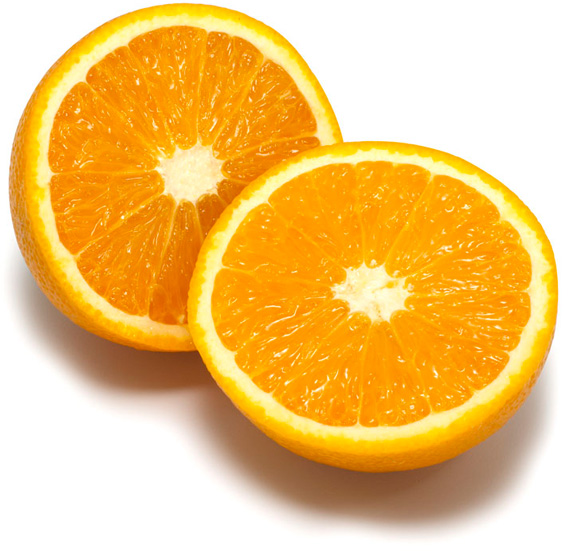
\includegraphics[scale=0.4]{../../bildat_lab3/orange.jpg}
  \caption{Image \texttt{orange}.}
  \label{fig:orange}
\end{figure}


\noindent\makebox[\textwidth][c]{%
\begin{minipage}{\linewidth}
  \begin{minipage}{0.45\linewidth}
    \begin{figure}[H]
      \centering
      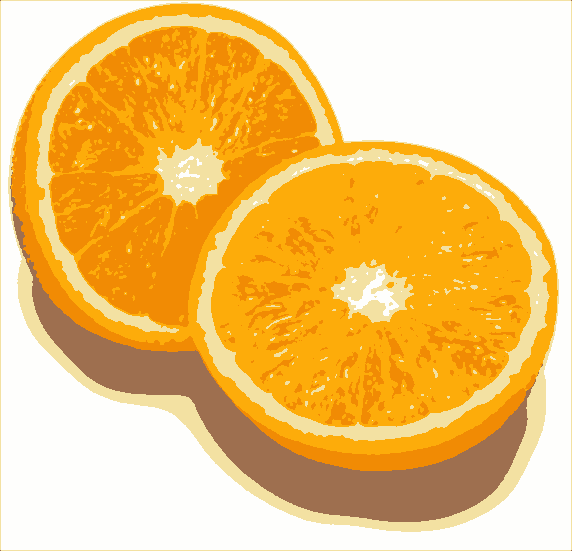
\includegraphics[scale=0.4]{./images/01/default1.png}
      \caption{Image \texttt{orange} segmented.}
      \label{fig:orange_segmented}
    \end{figure}
  \end{minipage}
  \hfill
  \begin{minipage}{0.45\linewidth}
    \begin{figure}[H]
      \centering
      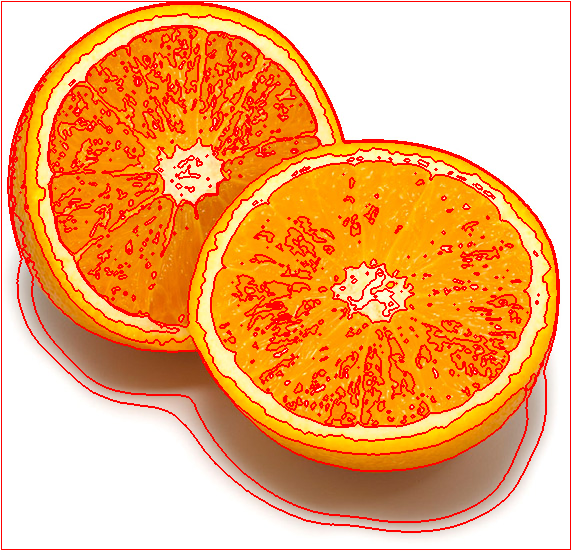
\includegraphics[scale=0.4]{./images/01/default2.png}
      \caption{Image \texttt{orange} and the bounds of its segments.}
      \label{fig:orange_segmented_bounds}
    \end{figure}
  \end{minipage}
\end{minipage}
}


% ------------------------------------------------------------------------------
% --------------------------------- Question 2 ---------------------------------
% ------------------------------------------------------------------------------
\subsection{Question 2}
Convergence time depends linearly on the number of clusters $K$ chosen and the
size of the image.
Furthermore it depends on the colour diversity of the image.
Tables \ref{tab:convergence_orange} and \ref{tab:convergence_tiger} illustrate
the number of iterations it takes for the k-means clustering method to
reach convergence depending on the number of clusters.

\begin{table}[H]
\centering
\makebox[0pt][c]{\parbox{\textwidth}{%
  \begin{minipage}[b]{0.45\hsize}\centering
    \begin{tabular}{c|c}
    $K$ & convergence iteration \\ \hline
    1                 & 2                     \\
    2                 & 9                     \\
    3                 & 14                    \\
    4                 & 11                    \\
    5                 & 18                    \\
    6                 & 21                    \\
    7                 & 17                    \\
    8                 & 35                    \\
    9                 & 46                    \\
    10                & 23                    \\
    11                & 38                    \\
    12                & 31                    \\
    \end{tabular}
    \caption{Number of centers $K$ and number of iterations taken to reach
      convergence with regard to image \texttt{orange}.
      \texttt{(scale\_factor, $\sigma$) $\equiv$ (1, 1)}}
    \label{tab:convergence_orange}
  \end{minipage}
  \hfill
  \begin{minipage}[b]{0.45\hsize}\centering
    \begin{tabular}{c|c}
      $K$ & convergence iteration \\ \hline
      1                 & 2                     \\
      2                 & 12                    \\
      3                 & 31                    \\
      4                 & 83                    \\
      5                 & 67                    \\
      6                 & 52                    \\
      7                 & 57                    \\
      8                 & 208                   \\
      9                 & 90                    \\
      10                & 103                   \\
      11                & 124                   \\
      12                & 132                   \\
    \end{tabular}
    \caption{Number of centers $K$ and number of iterations taken to reach
      convergence with regard to image \texttt{tiger1}.
      \texttt{(scale\_factor, $\sigma$) $\equiv$ (1, 1)}}
    \label{tab:convergence_tiger}
  \end{minipage}
}}
\end{table}


% ------------------------------------------------------------------------------
% --------------------------------- Question 3 ---------------------------------
% ------------------------------------------------------------------------------
\subsection{Question 3}

If I understand the question correctly, this value is $K=13$.
Figures \ref{fig:Q3:kmeans1_12} and \ref{fig:Q3:kmeans2_12} illustrate that
a superpixel covers parts from both halves of the orange for $K=12$,
whereas in figures \ref{fig:Q3:kmeans1_13} and \ref{fig:Q3:kmeans2_13},
where $K=13$, there is a clear boundary between them.

\noindent\makebox[\textwidth][c]{%
\begin{minipage}{\linewidth}
  \begin{minipage}{0.45\linewidth}
    \begin{figure}[H]
      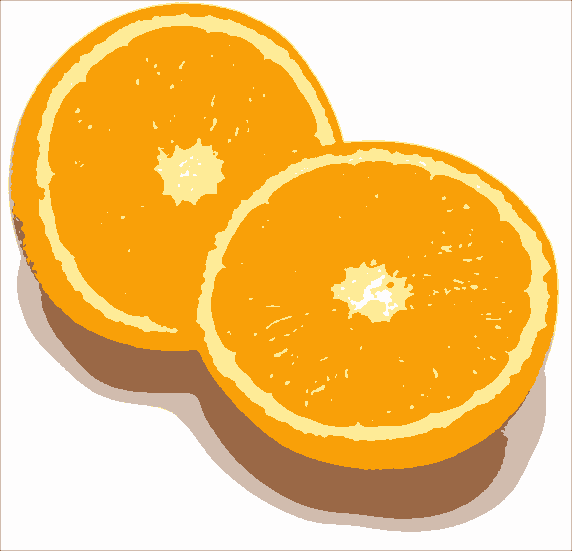
\includegraphics[scale=0.36]{./images/01/kmeans1_12.png}
      \caption{Image \texttt{orange} segmented using $K = 12$ clusters.}
      \label{fig:Q3:kmeans1_12}
    \end{figure}
  \end{minipage}
  \hfill
  \begin{minipage}{0.45\linewidth}
    \begin{figure}[H]
      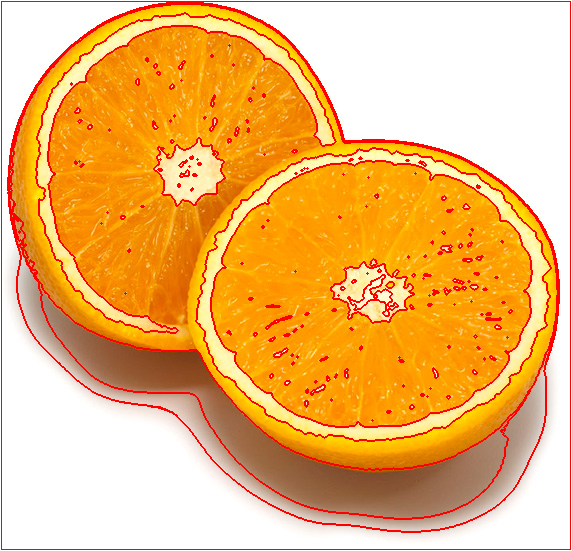
\includegraphics[scale=0.36]{./images/01/kmeans2_12.png}
      \caption{Image \texttt{orange} and the bounds of its segments for $K=12$.}
      \label{fig:Q3:kmeans2_12}
    \end{figure}
  \end{minipage}
\end{minipage}
}


\noindent\makebox[\textwidth][c]{%
\begin{minipage}{\linewidth}
  \begin{minipage}{0.45\linewidth}
    \begin{figure}[H]
      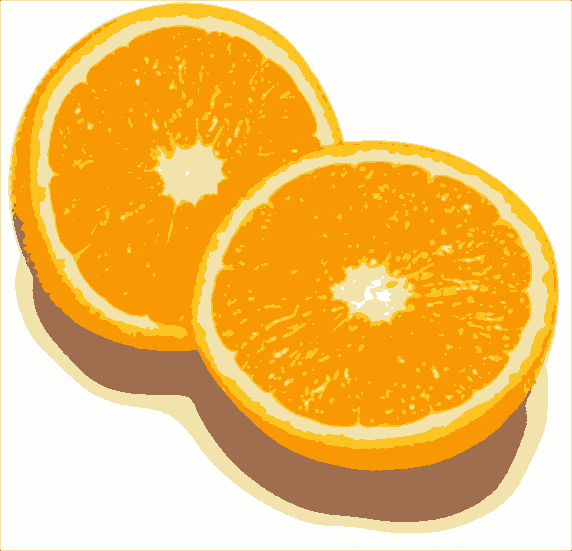
\includegraphics[scale=0.36]{./images/01/kmeans1_13.png}
      \caption{Image \texttt{orange} segmented using $K = 13$ clusters.}
      \label{fig:Q3:kmeans1_13}
    \end{figure}
  \end{minipage}
  \hfill
  \begin{minipage}{0.45\linewidth}
    \begin{figure}[H]
      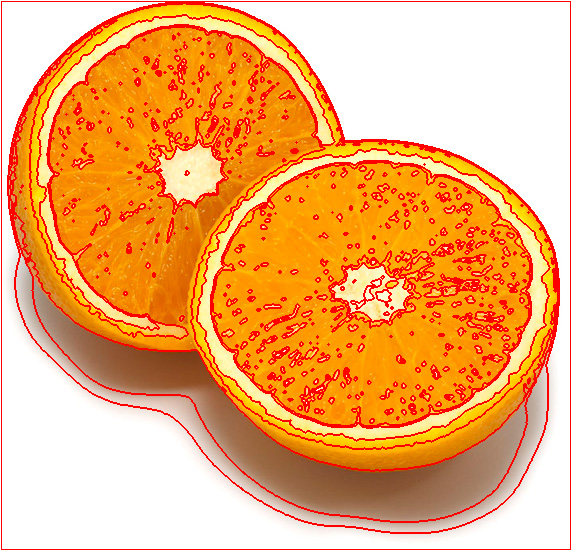
\includegraphics[scale=0.36]{./images/01/kmeans2_13.png}
      \caption{Image \texttt{orange} and the bounds of its segments for $K=13$.}
      \label{fig:Q3:kmeans2_13}
    \end{figure}
  \end{minipage}
\end{minipage}
}

% ------------------------------------------------------------------------------
% --------------------------------- Question 4 ---------------------------------
% ------------------------------------------------------------------------------
\subsection{Question 4}

Initially, what should be done is to increase the number of clusters $K$ since
image \texttt{tiger1} is more diverse in colour than image \texttt{orange}.
As convergence takes more iterations to be met for increasing number of clusters,
so should the iteration upper threshold $L$.

In the case where the clusters are not initialized in random but with a
certain colour set that is desired to be achieved, then the centers of these
clusters should be set to the values of those clusters.
